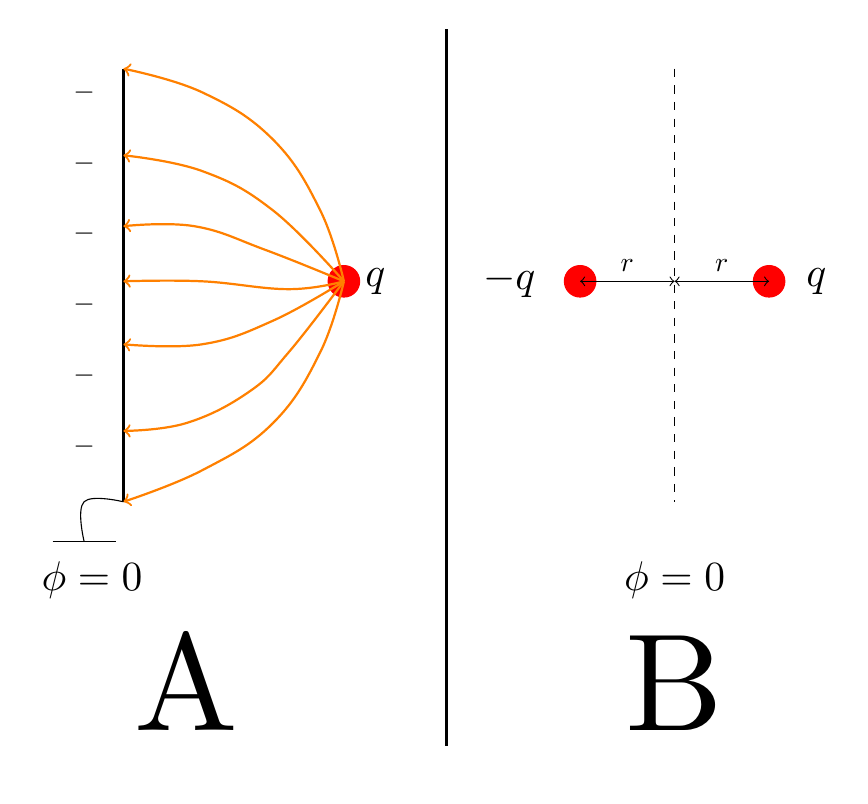
\begin{tikzpicture}

\draw [thick] (-2.5,3) node (v1) {} -- (-2.5,-2.5) node (v2) {};

\draw [dashed] (4.5,3) -- (4.5,-2.5);

\node (q) at (0.3,0.3) {};
\draw [fill, red] (q) circle [radius=0.2];
\draw [->, thick,orange] plot[smooth, tension=.7] coordinates {(q.center) (0,1.2) (-0.6,2.1) (-1.5,2.7) (v1)};
\draw  [->, thick,orange]plot[smooth, tension=.7] coordinates {(q.center) (0,-0.6) (-0.6,-1.5) (-1.5,-2.1) (v2)};
\draw  [->, thick,orange]plot[smooth, tension=.7] coordinates {(q.center) (-0.4,-0.6) (-0.9,-1.1) (-1.7,-1.5) (-2.5,-1.6)};
\draw  [->, thick,orange]plot[smooth, tension=.7] coordinates {(q.center) (-0.6,1.2) (-1.5,1.7) (-2.5,1.9)};
\draw  [->, thick,orange]plot[smooth, tension=.7] coordinates {(q.center) (-0.7,0.7) (-1.6,1) (-2.5,1)};
\draw [->, thick,orange] plot[smooth, tension=.7] coordinates {(q.center) (-0.6,-0.2) (-1.5,-0.5) (-2.5,-0.5)};
\draw  [->, thick,orange]plot[smooth, tension=.7] coordinates {(q.center) (-0.4,0.2) (-1.5,0.3) (-2.5,0.3)};
\node at (0.7,0.3) [black,scale=1.5] {$q$};
\node at (-2.9,-3.5) [black,scale=1.5] {$\phi=0$};
\node at (4.5,-3.5) [black,scale=1.5] {$\phi=0$};

\draw (-3.4,-3) -- (-2.6,-3);
\draw (-3.3,-3);
\node (q1) at (5.7,0.3) {};
\node (q2) at (3.3,0.3) {};
\draw [fill, red] (q1) circle [radius=0.2];
\draw [fill, red] (q2) circle [radius=0.2];
\node at (6.3,0.3) [black,scale=1.5] {$q$};
\node at (2.4,0.3) [black,scale=1.5] {$-q$};
\draw [<->](q2.center) -- (4.5,0.3) node [midway, above] (v3) {$r$};
\draw [<->](q1.center) -- (4.5,0.3) node [midway, above] {$r$};
\node at (-3,2.7) {$-$};
\node at (-3,1.8) {$-$};
\node at (-3,0.9) {$-$};
\node at (-3,0) {$-$};
\node at (-3,-0.9) {$-$};
\node at (-3,-1.8) {$-$};
\draw  plot[smooth, tension=.7] coordinates {(v2) (-3,-2.5) (-3,-3)};
\draw [very thick] (1.6,3.5) -- (1.6,-5.6);
\node at (-1.7,-4.8) [scale=5] {A};
\node at (4.5,-4.8) [scale=5] {B};
\end{tikzpicture}